\section{Handi Hermawan (1174080)}
\subsection{Instalasi Map Server}
\begin{enumerate}
    \item Pertama download aplikasi ms4w dahulu melalui website official ms4w.com
    \hfill\break
    \begin{figure}[H]
		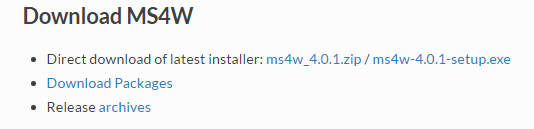
\includegraphics[width=4cm]{figures/tugas4/1174080/download.PNG}
		\centering
		\caption{Download MS4W}
    \end{figure}
    \hfill\break

    \item Tunggu proses install selesai (gunakan koneksi internet yang bagus)
    \hfill\break
    \begin{figure}[H]
		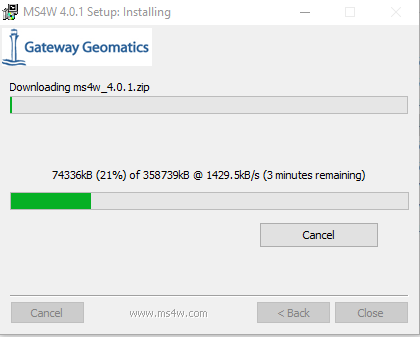
\includegraphics[width=4cm]{figures/tugas4/1174080/install_MS4W.PNG}
		\centering
		\caption{Proses Install}
    \end{figure}
    \hfill\break
    \item Proses instalan selesai
    \hfill\break
    \begin{figure}[H]
		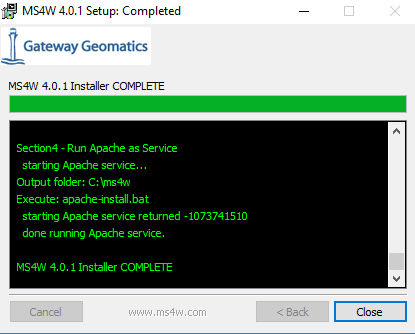
\includegraphics[width=4cm]{figures/tugas4/1174080/Selesai.PNG}
		\centering
		\caption{Install selesai}
    \end{figure}
    \hfill\break

\end{enumerate}

\subsection{Konfigurasi Map Server}
Setelah selesai melakukan instalasi kemudian konfigurasikan MS4W nya
\begin{enumerate}
  \item Buka Folder tempat anda install Mapserver4 lalu pergi ke folder ms4w kemudian apache lalu conf
  
  \item Buka file httpd.conf menggunakan editor favorit anda lalu ubah menjadi 1000 agar tidak konflik dengan XAMPP jika ada di komputer.
  
  \item Jika sudah buka services dengan menggunakan cmd
  \hfill\break
   
  \item Lalu pilih ApacheMS4WWebServer dan klik restart
  \hfill\break
  
\end{enumerate}

\subsection{Link Youtube Instalasi MapServer}
https://youtu.be/FU9tGvKfWqg

\subsection{Instalasi MapProxy}
\begin{enumerate}
  \item Buka CMD
  \item ketik pip install MapProxy
  \hfill\break
  \begin{figure}[H]
  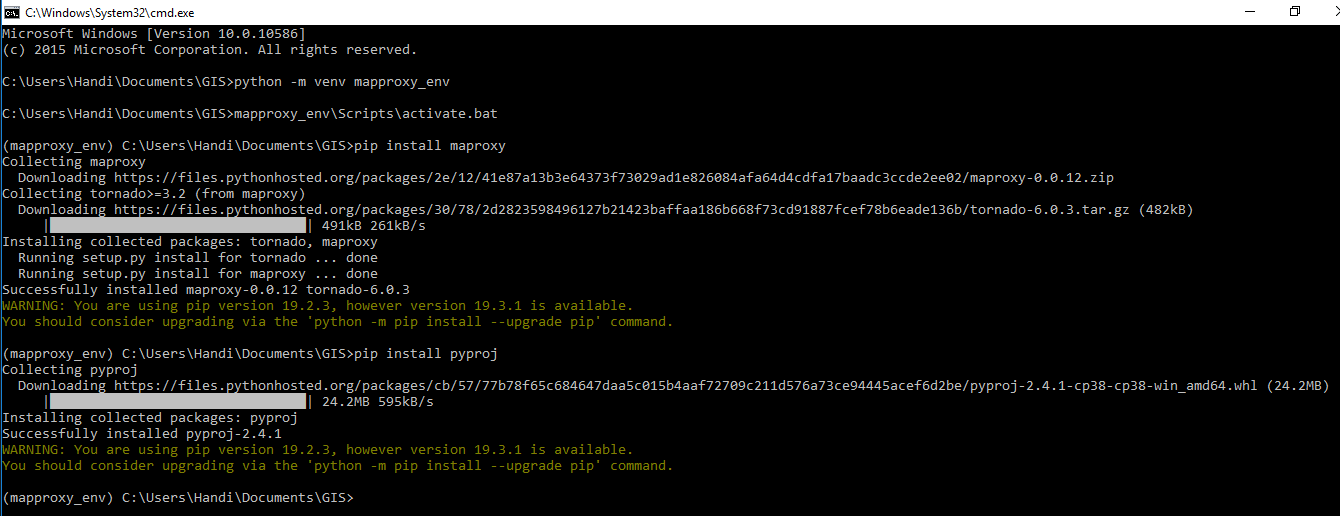
\includegraphics[width=4cm]{figures/tugas4/1174080/pip_proxy.PNG}
  \centering
  \caption{Instalasi MapProxy di cmd}
  \end{figure}
\end{enumerate}

\subsection{Membuka map menggunakan MapProxy}
\begin{enumerate}
  \item clone dulu git dari https://github.com/awangga/gede
  \item Pastikan path menuju folder gede tidak ada spasi contoh E:/gede-master
  \item Buat folder bernama tmp di gede-master
  \hfill\break
  \begin{figure}[H]
  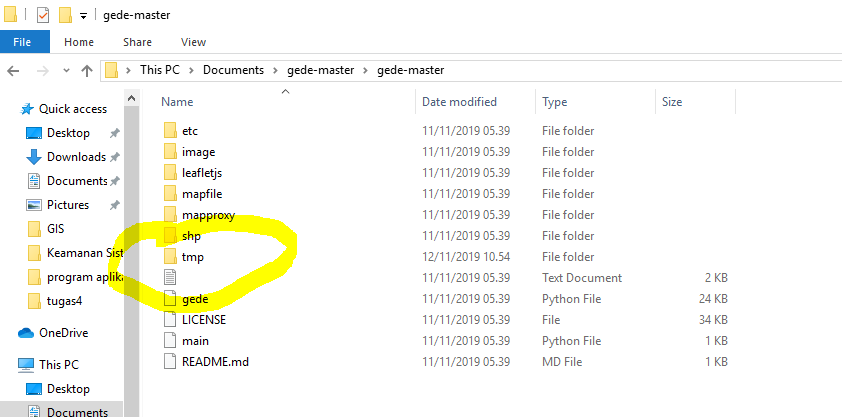
\includegraphics[width=4cm]{figures/tugas4/1174080/tmp.PNG}
  \centering
  \caption{Buat folder tmp}
  \end{figure}

  \item kemudian buka folder mapproxy lalu edit file agm.yaml
  \hfill\break
  \begin{figure}[H]
  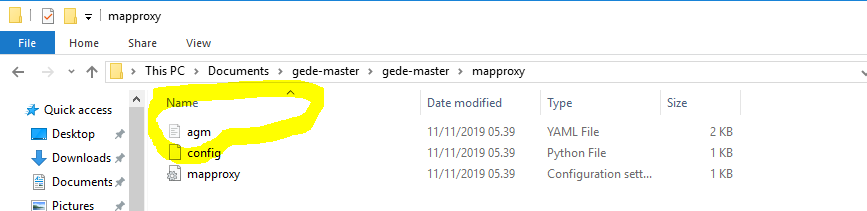
\includegraphics[width=4cm]{figures/tugas4/1174080/agm.PNG}
  \centering
  \caption{File agm.yaml}
  \end{figure}

  \item Pada bagian sources lalu ada map, masukkan pathnya sesuai dengan tempat direktori gede yang anda 
  \hfill\break
  \begin{figure}[H]
  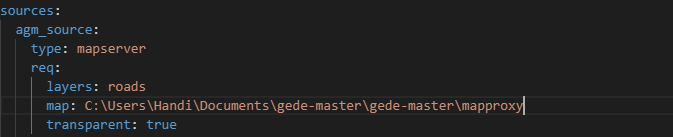
\includegraphics[width=4cm]{figures/tugas4/1174080/maymap.PNG}
  \centering
  \caption{Edit lokasi mymap.map}
  \end{figure}


  \item Lalu dibawahnya pada bagian binary masukkan lokasi instalasi ms4w anda
  \hfill\break
  \begin{figure}[H]
  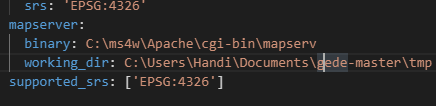
\includegraphics[width=4cm]{figures/tugas4/1174080/mapserv.PNG}
  \centering
  \caption{Edit path binary mapserv}
  \end{figure}


  \item setelah dibuka ketikkan "mapproxy-util serve-develop ./agm.yaml" pada ms4w-Shell untuk membuka aplikasi mapproxy
  \hfill\break
  \begin{figure}[H]
  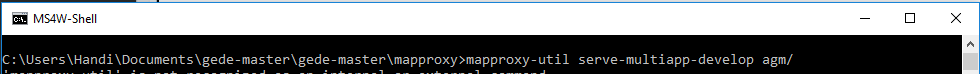
\includegraphics[width=4cm]{figures/tugas4/1174080/util.PNG}
  \centering
  \caption{Buka aplikasi mapproxy}
  \end{figure}
  
  \item Buka browser lalu ketikkan 127.0.0.1:8080
  \hfill\break
  \begin{figure}[H]
  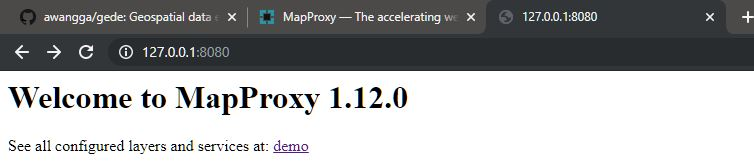
\includegraphics[width=4cm]{figures/tugas4/1174080/web.PNG}
  \centering
  \caption{Buka mapproxy pada browser}
  \end{figure}

  \item lalu klik demo untuk melihat map
  \item lalu klik png pada agm, maka mapproxy akan menampilkan map
  \hfill\break
  \begin{figure}[H]
  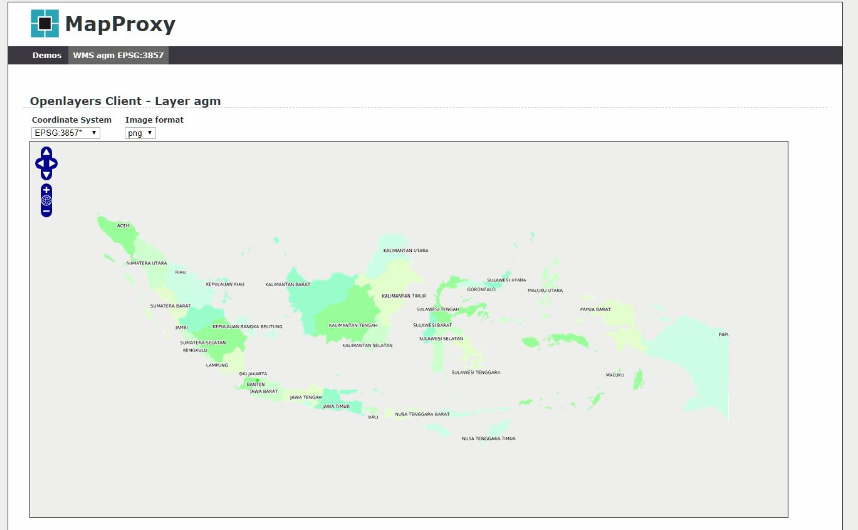
\includegraphics[width=4cm]{figures/tugas4/1174080/mapjadi.PNG}
  \centering
  \caption{MapProxy menampilkan map}
  \end{figure}

\end{enumerate}

\subsection{Link Youtube MapProxy dan Menjalankannya}
https://youtu.be/EW7SSOZUlZU